\documentclass[conference]{IEEEtran}
\IEEEoverridecommandlockouts
% The preceding line is only needed to identify funding in the first footnote. If that is unneeded, please comment it out.
\usepackage{cite}
\usepackage{amsmath,amssymb,amsfonts}
\usepackage{algorithmic}
\usepackage{graphicx}
\usepackage{textcomp}
\def\BibTeX{{\rm B\kern-.05em{\sc i\kern-.025em b}\kern-.08em
    T\kern-.1667em\lower.7ex\hbox{E}\kern-.125emX}}
\begin{document}

\title{Tour Miner:Mining System of Tour Plans from SNS\\
{\huge  --- Mining the User Experience into Travel Records ---}
}

\author{\IEEEauthorblockN{Shingo Yamaguchi, Katakura Shouta}
\IEEEauthorblockA{{Graduate School of Sciences and Technology for Innovation}  \\ 
Yamaguchi University\\
2-16-1 Tokiwadai, Ube 755-8611, Japan \\
Email: \{ fshingo, s055ffg \} @yamaguchi-u.ac.jp}
\and
\IEEEauthorblockN{Thanawit Gerdprasert, Anawat Kaenthong, \\Merisa Puengsawad}
\IEEEauthorblockA{{Department of Computer Engineering, Faculty of Engineering} \\
\textit{Kasetsart University}\\
Bangkok 10900, Thailand \\
Email : \{ thanawit.g, anawat.k, merisa.p \} }
\and
}

\maketitle

\begin{abstract}
Tour Miner is the process that consist of mining the tour plans from popular social network system when the given keyword is presented, the system then find the travel record from the according input and then return the Tour Record back to the user. 
While the previous paper, the research focus primarly on the Smelting process that use the heuristic mining in order to output the best possible tour record, in this paper we primarily focused on the mining function. We create the offline database which stored the user travel record in order to access it faster, the user input will be used to generate the travel record which will be used in the Smeltering function in the further part.
\end{abstract}

\section{Introduction}
With the popularity of the internet becoming more and more popular, the social network become relevant to our daily day life. People start using more and more social network system in order to share their own experience. This is where we proposed the Framework called Tour Miner (See  Fig. \ref{fig:overall}) which try to create the tour record based on the using the user experience from Social Network System. \par
Arai et al. [1] proposed the method of getting the travel record from social network system called Twitter and its support platform called Four Square in order to gather the user experience from the twitter using various keywords and notable term to improve the quality of the travel records by distributing the evaluation point into the user experience. The model from this research using the data from the twitter as the quality based, which result in the data that is very detailed and very valuable with the tradeoff to the lack of data amount. \par
For our research purpose, we want to emphasize on getting the numerous of travel record to improve the effective of the smeltering phase of the research. Alternatively, rather than gathering the record at the real time, we try to create the offline database in order to make our service process faster and suitable for recommending the tour plan for the user. In the final product, we plan to illustrate how the process work by develop the full-stack web application.

 \begin{figure}
  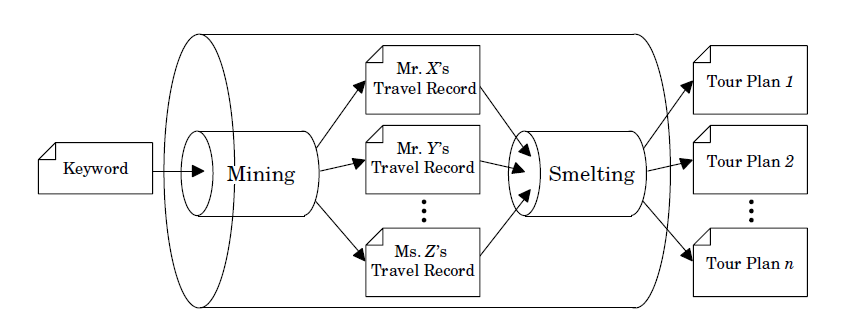
\includegraphics[width=\linewidth]{overall.png}
  \caption{Overall framework of the Tour Miner. This paper focus on the first part of the process called Web Mining.}
  \label{fig:overall}
\end{figure}

\section{Preminary}


\subsubsection{Tour Miner} Tour Miner is the process which has the goal to mines the tour plans from SNS. The framework consist of two main process, web mining  and process mining. Both of the process will be combined in order to generating the tour plan and deliver the result to the user.

\subsubsection{Web Mining} Web Mining is initial process of the tour miner system. The goal of this phase is to crawl and retrive the user experience from the SNS. The data preparation technique is then apply to the retrived data in order to make the data ready for the create and update the offline database. Offline database will allow us to perform querying with fast and effective to retrieve numerous of data to pass on the process mining.


\subsubsection{Process Mining}  Process mining techniques extract the knowledge from event logs to discover, monitor and improve processes. Process discovery is the most important technique. Distory technique takes an event log and produces a process model such as Petri Net and BPMN.


\section{Mining Function from Social Network System}

In this section, we elucidate the implementation of the mining function. We first illustrate the outline of the function and then detail of each step and detail of the function.

\subsubsection{Outline} 

Keep your text and graphic files separate until after the text has been 
formatted and styled. Do not number text heads---{\LaTeX} will do that 
for you.

\subsubsection{Getting Traveling User from SNS} 

\subsubsection{Create the traveling record for each user} 

\subsubsection{Storing user traveling record in the offline database} 

\section(Implementation and application example)



\section{Conclusion}

\section{References}

\textbf{The class file is designed for, but not limited to, six authors.} A 
minimum of one author is required for all conference articles. Author names 
should be listed starting from left to right and then moving down to the 
next line. This is the author sequence that will be used in future citations 
and by indexing services. Names should not be listed in columns nor group by 
affiliation. Please keep your affiliations as succinct as possible (for 
example, do not differentiate among departments of the same organization).

\subsection{Identify the Headings}
Headings, or heads, are organizational devices that guide the reader through 
your paper. There are two types: component heads and text heads.

Component heads identify the different components of your paper and are not 
topically subordinate to each other. Examples include Acknowledgments and 
References and, for these, the correct style to use is ``Heading 5''. Use 
``figure caption'' for your Figure captions, and ``table head'' for your 
table title. Run-in heads, such as ``Abstract'', will require you to apply a 
style (in this case, italic) in addition to the style provided by the drop 
down menu to differentiate the head from the text.

Text heads organize the topics on a relational, hierarchical basis. For 
example, the paper title is the primary text head because all subsequent 
material relates and elaborates on this one topic. If there are two or more 
sub-topics, the next level head (uppercase Roman numerals) should be used 
and, conversely, if there are not at least two sub-topics, then no subheads 
should be introduced.

\begin{thebibliography}{00}
\bibitem{b1} G. Eason, B. Noble, and I. N. Sneddon, ``On certain integrals of Lipschitz-Hankel type involving products of Bessel functions,'' Phil. Trans. Roy. Soc. London, vol. A247, pp. 529--551, April 1955.
\bibitem{b2} J. Clerk Maxwell, A Treatise on Electricity and Magnetism, 3rd ed., vol. 2. Oxford: Clarendon, 1892, pp.68--73.
\bibitem{b3} I. S. Jacobs and C. P. Bean, ``Fine particles, thin films and exchange anisotropy,'' in Magnetism, vol. III, G. T. Rado and H. Suhl, Eds. New York: Academic, 1963, pp. 271--350.
\bibitem{b4} K. Elissa, ``Title of paper if known,'' unpublished.
\bibitem{b5} R. Nicole, ``Title of paper with only first word capitalized,'' J. Name Stand. Abbrev., in press.
\bibitem{b6} Y. Yorozu, M. Hirano, K. Oka, and Y. Tagawa, ``Electron spectroscopy studies on magneto-optical media and plastic substrate interface,'' IEEE Transl. J. Magn. Japan, vol. 2, pp. 740--741, August 1987 [Digests 9th Annual Conf. Magnetics Japan, p. 301, 1982].
\bibitem{b7} M. Young, The Technical Writer's Handbook. Mill Valley, CA: University Science, 1989.
\end{thebibliography}

\end{document}
